\chapter{Abordagem Proposta} \label{chap:propApproach}
	\begin{myenv}{1.5}
		\section{Coleta de dados}
			\par Para a realização desta pesquisa coletou-se uma série de vozes nos arredores do Instituto de Biociências, Letras e Ciências Exatas em São José do Rio Preto no estado de São Paulo. Foram coletadas amostras de 21 Indivíduos, das quais 20 foram usadas já que, em um dos casos, não foi possível coletar todos os dados necessários. Tais gravações se constituem de dígitos em um intervalo de 0 a 9 falados tanto em língua inglesa como em portuguesa. Os locutores foram escolhidos de acordo com seu sexo e idade de forma que a amostra estudada tenha uma abrangência que cubra desde crianças em época pré-escolar até adultos entre 50 e 60 anos do sexo masculino e feminino.
						
			\par As gravações foram feitas em ambientes distintos com diferentes níveis de ruído ao fundo garantindo uma boa variabilidade de interferências que certamente irão impactar nos resultados dos classificadores que serão usados.
			
			\par Coletadas as amostras, os dígitos das mesmas foram separados um-a-um usando uma ferramenta desenvolvida para esse fim, resultando em uma base de dados com 820 trechos. No apêndice deste documento é possível entender a ferramenta criada para auxiliar na preparação desta base de dados.
			
			\subsection{Base de dados de áudios originais}
				\par Para a constituição da base de dados não regravada os áudios originais foram editados e separados digito a dígito.
	
			\subsection{Base de dados de áudios regravados}
				\par No caso da base usada para simulação de \textit{voice spoofing} foi criado um arquivo contendo todas as falas de todos os entrevistados, em seguida, os sons reproduzidos por este foram regravados por um segundo dispositivo de gravação diferente do original.

			\subsection{Organização}
				\par A organização da base de dados se deu por tipo (regravado ou não), idioma, dígito ditado e interlocutor considerado. Foi criada uma estrutura hierárquica de diretórios de forma a permitir que fosse fácil e intuitivo acessar cada uma das amostras seja por vias automatizadas ou não. Os arquivos regravados residem no diretório "playback" \ já os não regravados se encontram em "live".	Essa organização é mostrada nas figuras \ref{fig:directorystructlevel01}, \ref{fig:directorystructlevel02} e \ref{fig:directorystructlevel03}.
				
				\par Para facilitar a automação do processamento foram criados três arquivos de texto:
				\begin{itemize}
					\item \textit{\textbf{dataSurvey.txt}}: Contêm os dados de idade e sexo de cada entrevistado.
					\item \textit{\textbf{inputListLive.txt}}: Uma lista de caminhos para todos os arquivo não regravados.
					\item \textit{\textbf{inputListSpoofing.txt}}: Apresenta uma listagem dos caminhos para todos os arquivos regravados.
				\end{itemize}
			
				\par Apenas para ilustrar, o conteúdo do diretório \textbf{"separated \textfractionsolidus live \textfractionsolidus en\_US \textfractionsolidus 0"} se constitui de vários arquivos do tipo \textit{wave} cada um identificando o locutor ao qual pertence como mostrado na  figura \ref{fig:directorystructlevel03}.
					
				\begin{figure}
					\center
					\subfigure[Base em nível 1]{
						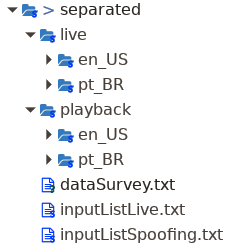
\includegraphics{images/directoryStructLevel01}
						\label{fig:directorystructlevel01}
					}
					\subfigure[Base em nível 2]{
						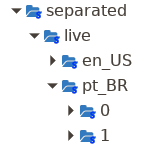
\includegraphics{images/directoryStructLevel02}
						\label{fig:directorystructlevel02}
					}
					\subfigure[Base em nível 3]{
						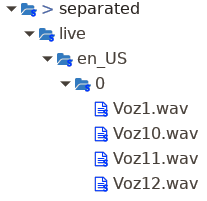
\includegraphics{images/directoryStructLevel03}
						\label{fig:directorystructlevel03}
					}
					\caption{Organização da base de dados}
					\label{fig:directorystructlevel010203}
				\end{figure}

		\section{Experimentos}
			\subsection{Experimento 01 - Melhor combinação Wavelet x BARK ou MEL}
				\subsubsection{Apresentação}
					\par O objetivo desse experimento verificar, segundo análise paraconsistente, qual das combinações entre as escalas BARK ou MEL e as várias \textit{wavelets} consideradas geram os vetores de características com menos sobreposição (disjuntos).
					
					\par Mais informações sobre a análise paraconsistente se encontram no capítulo \ref{chap:revBibli}. 
					
					\par O uso de \textit{wavelets} geralmente tem como objetivo a geração de vetores que serão analisados ou processados posteriormente, tais sequências de valores carregam a informação de frequência e tempo que podem ser úteis para uma análise específica. Neste trabalho, porém, a decomposição deve ser feita até seu limite, pois, após isso será realizada a soma das energias nos intervalos definidos pela escala BARK e MEL que seriam impossíveis, ou imprecisas se assim não fosse. Por fim, é feito o posicionamento dos resultados no plano paraconsistente.
					
					\par O algoritmo para a realização das etapas é mostrado na listagem \ref{lst:experiment01Algo}.
				
				\subsubsection{Redimensionando o sinal}
					\par Antes da aplicação da transformada \textit{wavelet} é necessário redimensionar o sinal para que este tenha um comprimento correspondente a uma potência de 2 como indicado na equação \ref{eq:optimalSize}. Isso é necessário para que não haja perdas de informação ao final da transformação, pois, como a transformada \textit{wavelet} realiza o \textit{downsampling} numa ordem de 2, ou seja, em cada nível o tamanho do vetor do sinal é diminuído pela metade. Caso haja um comprimento diferente do citado, em alguma parte do processo a divisão não será inteira fazendo com que algum/alguns valores dentro do processamento não sejam considerados.
					
					\par Na equação \ref{eq:optimalSize} \textit{\textbf{proxInt}} é uma função que retorna o próximo número inteiro dado outro real (por exemplo, $proxInt(1,5) = 2$) e \textit{\textbf{tamanho}} é a quantidade de itens no vetor do sinal.

					\begin{equation}
						tamanhoOtimo=2^{proxInt(\log_{2}tamanho)}
						\label{eq:optimalSize}
					\end{equation} 
				
				\subsubsection{Determinando o número máximo de transformações}
					\par Após o redimensionamento do sinal a quantidade máxima de transformações necessárias para reduzir os coeficientes a um vetor unitário é dada pela equação \ref{eq:maxWaveletTransf}. 
					
					\begin{equation}
						maxTrans=\log_{2}tamanho
						\label{eq:maxWaveletTransf}
					\end{equation}
	
				\subsubsection{Wavelets testadas}
					\par Foram testadas as seguintes wavelets:
					\begin{multicols}{5}
						\begin{itemize}
							\item haar		\item daub4		\item daub6		\item daub8
							\item daub10	\item daub12	\item daub14	\item daub16
							\item daub18	\item daub20	\item daub22	\item daub24
							\item daub26	\item daub28	\item daub30	\item daub32
							\item daub34	\item daub36	\item daub38	\item daub40
							\item daub42	\item daub44	\item daub46	\item daub48
							\item daub50	\item daub52	\item daub54	\item daub56
							\item daub58	\item daub60	\item daub62	\item daub64
							\item daub66	\item daub68	\item daub70	\item daub72
							\item daub74	\item daub76	\item sym8		\item sym16
							\item sym32		\item coif6		\item coif12	\item coif18
							\item coif24	\item coif30	\item beylkin18	\item vaidyanathan24
						\end{itemize}
					\end{multicols}
				\subsubsection{Algoritmo}
				\begin{lstlisting}[language=C++]
// Carregue para a memoria um dos conjuntos de amostra
for (listaDeAmostras : {listaComVoiceSpoofing, listaSemVoiceSpoofing}) {
	// Selecione o proximo tipo de wavelet
	for (wavelet : wavelets) {
		// Selecione entre BARK ou MEL
		for (barkOuMel : {BARK, MEL}) {
			// Selecione o proximo sinal dentro da amostra
			for (sinal : listaDeAmostras) {
				tamanhoOtimo=calcularTamanhoOtimo(sinal);
				redimensionar(sinal, tamanhoOtimo);
				sinalTransformado=wavelet(sinal, wavelet);
				energias=calcularEnergias(sinalTransformado, barkOuMel);
				energias=normalizar(energias);
				
				// Armazene os resultados
				resultados[wavelet.nome()][barkOuMel][listaDeAmostras.nome()].adicionar(energias);
			}
		}
	}
}
// Posicione os resultados no plano paraconsistente
mostraResultadosNoPlanoParaconsistente(resultados);
\end{lstlisting}

			\subsection{Experimento 02 - Desempenho da combinação mais disjunta em classificadores por distância.}
				\subsubsection{Apresentação}
					\par O objetivo deste é verificar, considerando as melhores combinações descobertas pelo experimento 1, o desempenho de classificadores por distâncias Euclidiana e Manhattan. Nesta fase do estudo os vetores de características gerados pelo experimento 1 são fornecidos aos classificadores cujos desempenhos serão medidos.
					
					\par Objetivando medir o comportamento da classificação com diversos tamanhos para os modelos de referência, o tamanho dos mesmos foi definido segundo porcentagens da quantidade total de amostras.
					
					\par Para cada porcentagem escolhida o experimento deve ser uma vez, depois duas vezes, após isso 3, 4, 5, até que se chegue a execução de um número definido de testes dado pela equação \ref{eq:amountOftests}. Em cada uma dessas execuções, a ordem dos sinais dentro das amostras (\textit{spoofing} e não \textit{spoofing}) foi permutada aleatoriamente para evitar que uma coincidência afetasse os valores dos resultados.
					
					\par Abaixo: \textit{\textbf{numTestes}} representa número máximo de testes que podem ser feitos usando uma certa porcentagem.
					\begin{equation}
						\label{eq:amountOftests}
						qtdeTotalDeTestes= numTestes * \dfrac{numTestes + 1}{2}
					\end{equation}
					
					\par Para cada porcentagem foram coletadas as melhores e as piores acurácias assim como suas respectivas matrizes de confusão.
					
					\par O algoritmo deste experimento é mostrado na listagem \ref{lst:experiment02Algo}.
									
				\subsubsection{Amostragem}
					\par Houve uma separação entre amostras para teste e outras constituir o modelo de referência para o classificador. Os modelos de referência foram dimensionados usando-se 10\%, 20\%, 30\%, 40\% e 50\% da quantidade total de amostras para ambas as classes (\textit{spoofing} e não \textit{spoofing}) as restantes foram usadas nos testes.	
				\subsubsection{Algoritmo}
				\begin{lstlisting}[language=C++, caption={Procedure 02 algorithm}, label={lst:experiment02Algo}]
modelProportion={0.1, 0,2, 0,4, 0,5};
genuineModel = spoofingModel= genuineTest = spoofingTest = accuracyList = {};
for (distance : {Euclidian, Manhattan}) {
	for(percentage : modelProportion){
		for(testCounter = 0; testCounter < 300; testCounter++){
			// Choose feature vectors randomly from spoofing set
			// to build the model according to the proportions chosen.
			chooseRamdomly(voiceSpoofingSet, percentage, spoofingModel, spoofingTest);
			// Choose feature vectors randomly from genuine set
			// to build the tests according to the proportion chosen
			chooseRamdomly(genuineSet, percentage, genuineModel, genuineTest);
			
			trainClassificator("spoofing", spoofingModel);
			trainClassificator("genuine", genuineModel);
			// Classify the spoofing tests against the 
			// spoofing model and fill the confusion tables
			for(signal : spoofingTest){
				fillConfusionTable(signal, "spoofing");
			} 
			// Classify the genuine tests against the
			// genuine model and fill the confusion tables
			for(signal : genuineTest){
				fillConfusionTable(signal, "genuine");
			}

			accuracy=calculateAccuracy();
			
			// Store the accuracies for each percentage
			accuracyList[percentage].add(accuracy);

			// Store the best accuracy and its respective confusion table
			if(isTheBestAccuracy(accuracy)){
				saveAccuracyAndItsConfusionTable();
			}
			
			// Store the worst accuracy and its respective confusion table
			if(isTheWorstAccuracy(accuracy)){
				saveAccuracyAndItsConfusionTable();
			}
		}
		
		// Calculate and save the standard deviation for current proportion
		calculateAndSaveTheStandardDeviation(accuracyList[percentage]);
	}
}				
\end{lstlisting}

			\subsection{Experimento 03 - Desempenho da combinação mais disjunta em uma SVM.}
				\subsubsection{Apresentação}
					\par Considerando as melhores combinações descobertas pelo experimento 1, nesta parte pretende-se medir o desempenho de uma \textit{Support Vector Machine} (SVM). Nesta fase do estudo os vetores de características gerados pelo experimento 1 são fornecidos ao classificador cujo desempenho será medido. São idênticas ao experimento 2 as quantidades de testes, as formas de separação dos conjuntos de modelo e teste (amostragem), assim como boa porção do algoritmo, este, será apresentado apenas como garantia do entendimento e se encontra na listagem \ref{lst:experiment03Algo}.

				\subsubsection{Algoritmo}
				\begin{lstlisting}[language=C++, caption={Algoritmo que caracteriza o procedimento 03}, label={lst:experiment03Algo}]
tamanhosDoModelo={0.1, 0,2, 0,4, 0,5};
modeloDeReferenciaNaoSpoofing={};
modeloDeReferenciaSpoofing={};
testesNaoSpoofing={};
testesSpoofing={};
	for(porcentagem : tamanhosDoModelo){
		for(teste = 0; teste < 300; teste++){
			// Escolhe aleatoriamente os sinais para o modelo com spoofing 
			// e os grava em 'modeloDeReferenciaSpoofing' o restante vai 
			// para 'testesSpoofing'
			escolherAleatoriamente(listaComVoiceSpoofing, porcentagem, modeloDeReferenciaSpoofing, testesSpoofing);
			
			// Escolhe aleatoriamente os sinais para o modelo sem spoofing
			// e os grava em 'modeloDeReferenciaNaoSpoofing' o restante vai 
			// para 'testesNaoSpoofing'
			escolherAleatoriamente(listaSemVoiceSpoofing, porcentagem, modeloDeReferenciaNaoSpoofing, testesNaoSpoofing);
			treinarClassificador("spoofing", modeloDeReferenciaSpoofing);
			treinarClassificador("naoSpoofing", modeloDeReferenciaNaoSpoofing);
			
			// Classifica os testes e preenche a tabela de confusao
			for(sinal : testesSpoofing){
				preencherTabelaDeConfusao(sinal, "spoofing");
			} 
			
			// Classifica os testes e preenche a tabela de confusao
			for(sinal : testesNaoSpoofing){
				preencherTabelaDeConfusao(sinal, "naoSpoofing");
			}
			
			acuracia=calculaAcuracia();
			
			// Salva a melhor acuracia e matriz de confusao
			if(ehAMelhorAcuracia(acuracia)){
				salvaAcuraciaEMatrizDeConfusao();
			}
			
			// Salva a pior acuracia e matriz de confusao
			if(ehAPiorAcuracia(acuracia)){
				salvaAcuraciaEMatrizDeConfusao();
			}
		}
	}			
\end{lstlisting}
	\end{myenv}